%%%%%%%%%%%%%%%%%%%%%%%%%%%%%%%%%%%%%%%%%
% Arsclassica Article
% LaTeX Template
% Version 1.1 (05/01/2015)
%
% This template has been downloaded from:
% http://www.LaTeXTemplates.com
%
% Original author: Adriano Palombo
%
%
%%%%%%%%%%%%%%%%%%%%%%%%%%%%%%%%%%%%%%%%%

%----------------------------------------------------------------------------------------
%	PACKAGES AND OTHER DOCUMENT CONFIGURATIONS
%----------------------------------------------------------------------------------------

\documentclass[
11pt, % Main document font size
a4paper, % Paper type, use 'letterpaper' for US Letter paper
oneside, % One page layout (no page indentation)
%twoside, % Two page layout (page indentation for binding and different headers)
headinclude,footinclude, % Extra spacing for the header and footer
BCOR5mm, % Binding correction
]{scrartcl}

%%%%%%%%%%%%%%%%%%%%%%%%%%%%%%%%%%%%%%%%%
% Arsclassica Article
% Structure Specification File
%
% This file has been downloaded from:
% http://www.LaTeXTemplates.com
%
% Original author:
% Lorenzo Pantieri (http://www.lorenzopantieri.net) with extensive modifications by:
% Vel (vel@latextemplates.com)
%
% License:
% CC BY-NC-SA 3.0 (http://creativecommons.org/licenses/by-nc-sa/3.0/)
%
%%%%%%%%%%%%%%%%%%%%%%%%%%%%%%%%%%%%%%%%%

%----------------------------------------------------------------------------------------
%	REQUIRED PACKAGES
%----------------------------------------------------------------------------------------

\usepackage[
nochapters, % Turn off chapters since this is an article        
beramono, % Use the Bera Mono font for monospaced text (\texttt)
eulermath,% Use the Euler font for mathematics
pdfspacing, % Makes use of pdftex’ letter spacing capabilities via the microtype package
dottedtoc % Dotted lines leading to the page numbers in the table of contents
]{classicthesis} % The layout is based on the Classic Thesis style

\usepackage{arsclassica} % Modifies the Classic Thesis package

\usepackage[T1]{fontenc} % Use 8-bit encoding that has 256 glyphs

\usepackage[utf8]{inputenc} % Required for including letters with accents
\usepackage[british,UKenglish]{babel}
\usepackage{graphicx} % Required for including images
\graphicspath{{Figures/}} % Set the default folder for images

\usepackage{enumitem} % Required for manipulating the whitespace between and within lists

\usepackage{lipsum} % Used for inserting dummy 'Lorem ipsum' text into the template

\usepackage{subfig} % Required for creating figures with multiple parts (subfigures)

\usepackage{amsmath,amssymb,amsthm} % For including math equations, theorems, symbols, etc

\usepackage{varioref} % More descriptive referencing

%----------------------------------------------------------------------------------------
%	THEOREM STYLES
%---------------------------------------------------------------------------------------

\theoremstyle{definition} % Define theorem styles here based on the definition style (used for definitions and examples)
\newtheorem{definition}{Definition}

\theoremstyle{plain} % Define theorem styles here based on the plain style (used for theorems, lemmas, propositions)
\newtheorem{theorem}{Theorem}

\theoremstyle{remark} % Define theorem styles here based on the remark style (used for remarks and notes)

%----------------------------------------------------------------------------------------
%	HYPERLINKS
%---------------------------------------------------------------------------------------

\hypersetup{
%draft, % Uncomment to remove all links (useful for printing in black and white)
colorlinks=true, breaklinks=true, bookmarks=true,bookmarksnumbered,
urlcolor=webbrown, linkcolor=RoyalBlue, citecolor=webgreen, % Link colors
pdftitle={}, % PDF title
pdfauthor={\textcopyright}, % PDF Author
pdfsubject={}, % PDF Subject
pdfkeywords={}, % PDF Keywords
pdfcreator={pdfLaTeX}, % PDF Creator
pdfproducer={LaTeX with hyperref and ClassicThesis} % PDF producer
} % Include the structure.tex file which specified the document structure and layout

\hyphenation{Fortran hy-phen-ation} % Specify custom hyphenation points in words with dashes where you would like hyphenation to occur, or alternatively, don't put any dashes in a word to stop hyphenation altogether

%----------------------------------------------------------------------------------------
%	TITLE AND AUTHOR(S)
%----------------------------------------------------------------------------------------

\title{\normalfont\spacedallcaps{User Manual}} % The article title

\author{\spacedlowsmallcaps{Ryan Naidoo}} % The article author(s) - author affiliations need to be specified in the AUTHOR AFFILIATIONS block

\date{} % An optional date to appear under the author(s)

%----------------------------------------------------------------------------------------

\begin{document}

%----------------------------------------------------------------------------------------
%	HEADERS
%----------------------------------------------------------------------------------------

\renewcommand{\sectionmark}[1]{\markright{\spacedlowsmallcaps{#1}}} % The header for all pages (oneside) or for even pages (twoside)
%\renewcommand{\subsectionmark}[1]{\markright{\thesubsection~#1}} % Uncomment when using the twoside option - this modifies the header on odd pages
\lehead{\mbox{\llap{\small\thepage\kern1em\color{halfgray} \vline}\color{halfgray}\hspace{0.5em}\rightmark\hfil}} % The header style

\pagestyle{scrheadings} % Enable the headers specified in this block

%----------------------------------------------------------------------------------------
%	TABLE OF CONTENTS & LISTS OF FIGURES AND TABLES
%----------------------------------------------------------------------------------------

\maketitle % Print the title/author/date block

\setcounter{tocdepth}{2} % Set the depth of the table of contents to show sections and subsections only

\tableofcontents % Print the table of contents

\listoffigures % Print the list of figures

%\listoftables % Print the list of tables

%----------------------------------------------------------------------------------------
%	AUTHOR AFFILIATIONS
%----------------------------------------------------------------------------------------

%{\let\thefootnote\relax\footnotetext{* \textit{SireSLA, Lombardia Informatica, Milano, Italia}}}

%{\let\thefootnote\relax\footnotetext{\textsuperscript{1} \textit{Department of Chemistry, University of Examples, London, United Kingdom}}}

%----------------------------------------------------------------------------------------

\newpage % Start the article content on the second page, remove this if you have a longer abstract that goes onto the second page

%----------------------------------------------------------------------------------------
%	INTRODUCTION
%----------------------------------------------------------------------------------------

\section{Parameter Estimation for Chan-Vese Segmentation for Fluorescence Microscopy GUI}

\begin{enumerate}
\item When the application is executed, the interface will like the figure below
\begin{figure}[h]
\centering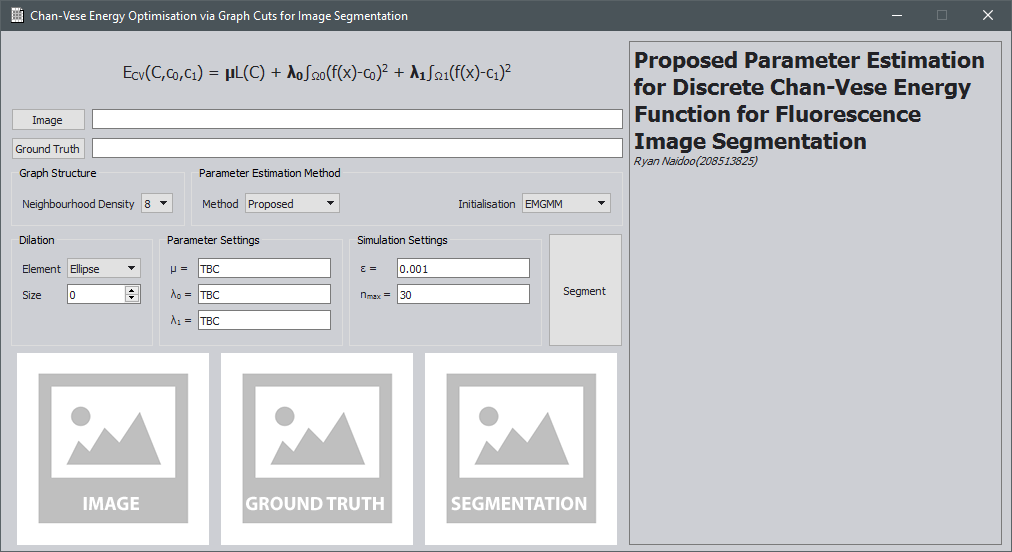
\includegraphics[width=0.90\columnwidth]{CVParamsEstimationGUI/OnStartup_raw}
\caption{On startup.}
\end{figure}

\item
Load in an image by clicking on the button labelled "Image" an image explorer dialogue will open as shown in the figure below. Then navigate to the desired image.
\begin{figure}[h]
	\centering
	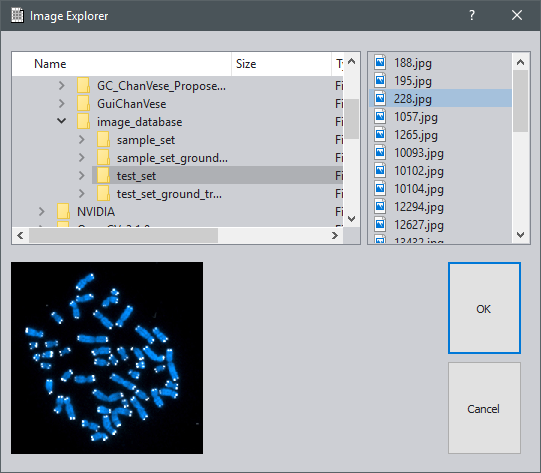
\includegraphics[width=0.90\columnwidth]{CVParamsEstimationGUI/OnImageNavigation}
	\caption{Image explorer to load an image.}
\end{figure}

\item 
When an image has been succesfully loaded it will appear in its designate slot as shown in the figure below.
\begin{figure}[h]
\centering
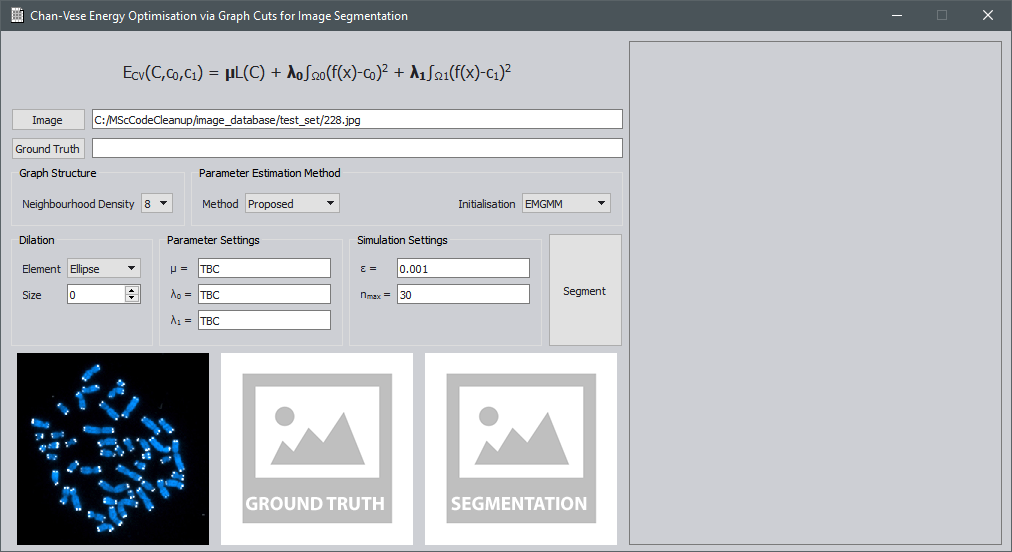
\includegraphics[width=0.90\columnwidth]{CVParamsEstimationGUI/afterImageNavigation}
\caption{Sucessfully loaded image.}
\end{figure}

%\newpage
\item 
\textit{Optional} Load a ground truth image by clicking on the button labelled "Ground Truth", an image explorer dialogue will open as shown in the figure below. Then navigate to the desired image.
\begin{figure}[h]
	\centering
	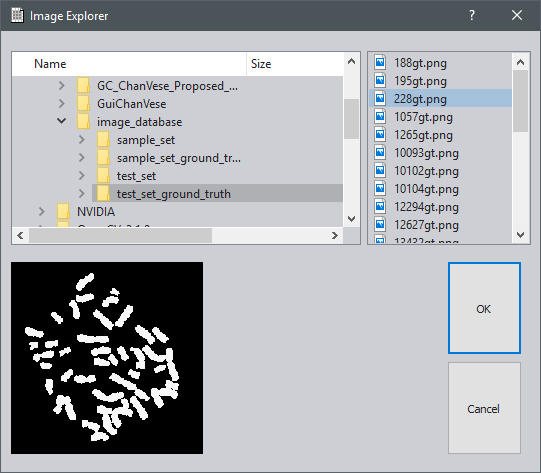
\includegraphics[width=0.90\columnwidth]{CVParamsEstimationGUI/OnGTNavigation}
	\caption{Image explorer to load a ground truth image.}
\end{figure}

\item
When a ground truth image has been succesfully loaded it will appear in its designate slot as shown in the figure below.
\begin{figure}[h]
	\centering
	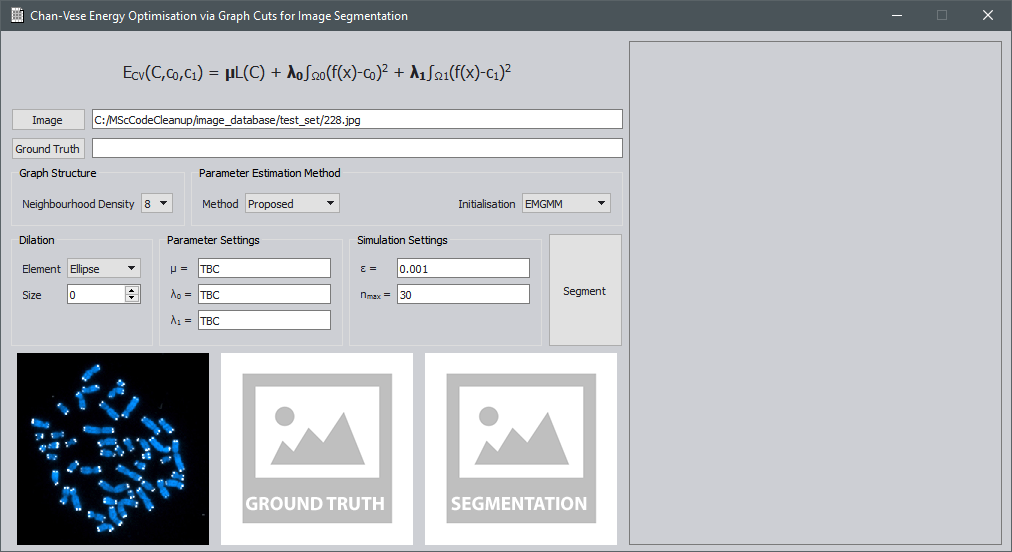
\includegraphics[width=0.90\columnwidth]{CVParamsEstimationGUI/afterImageNavigation}
	\caption{Sucessfully loaded image.}
\end{figure}
\newpage
\item Set the segmentation parameters. All list parameters are shown in the figure below.
\begin{enumerate}
	\item[$\bullet$]
	\textit{Neighbourhood Density} is the connectivity density of the graph to be built. The only options are 4-connected and 8-connected (default).
	
	\item[$\bullet$]
	\textit{Method} determines the type of parameter estimation method to use. The options are the parameter settings by El-Zehiry \textit{et. al} and Masaka \textit{et. al}, the proposed parameter estimation method (default) and manual tuning to allow for user-defined parameter settings.
	
	\item[$\bullet$]
	\textit{Initialisation} is the initial curve/mask which is iteratively deformed until convergence. The options are a centred circle, and curves/masks generated by Otsu binarizartion, K-means clustering ($k=2$) and EMGMM (Expectation Maximisation Gaussian Mixture Modelling with k=2) (default).
	
	\item[$\bullet$]
	\textit{Element} is the dilation element to be used on the initial curve/mask. The options are Rectangle, Cross, and Ellipse.
	
	\item[$\bullet$]
	\textit{Size} denotes the size of the dilation element in pixels. By default, no dilation is applied.
	
	\item[$\bullet$]
	\textit{Energy function parameters, $\mu$, $\lambda_0$ and $\lambda_1$}, are automatically calculated and shown in the designated text boxes. If "Manual" method is chosen then these can be edited by the user.
	
	\item[$\bullet$]
	\textit{Simulation Settings} cover the extra settings for segmentation. The convergence criterion is shown as $\epsilon$ which is set to $0.001$ by default, and the maximum number of iterations is shown as $n_{max}$ which is set to $30$ by default.
\end{enumerate}
\begin{figure}[h]
	\centering
	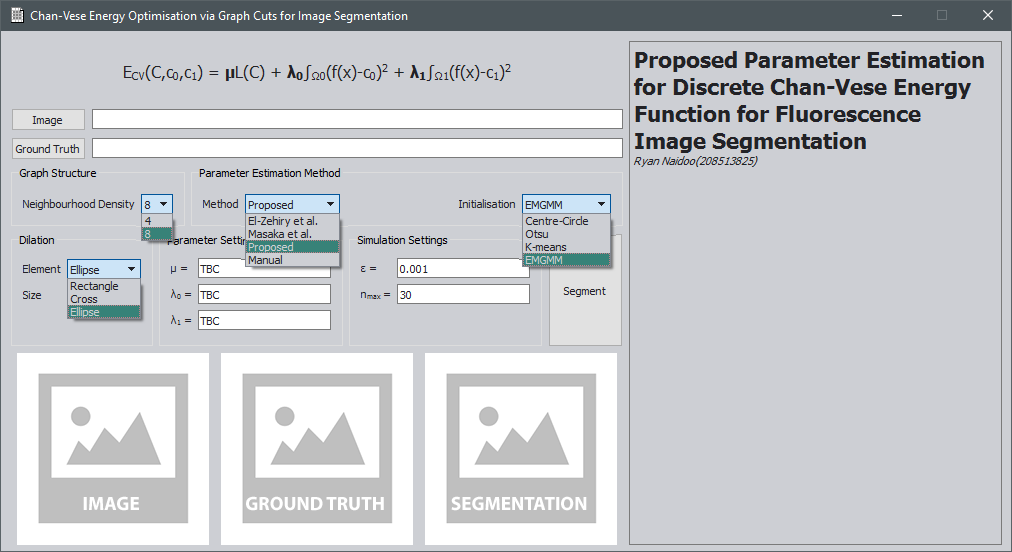
\includegraphics[width=0.90\columnwidth]{CVParamsEstimationGUI/all_parameters}
	\caption{All list parameters exposed.}
\end{figure}
\newpage
\item
Click the "Segment" button to start segmenting with the chosen parameters. A summary will appear on the segmentation results box as shown in the figure below.
\begin{figure}[h]
\centering
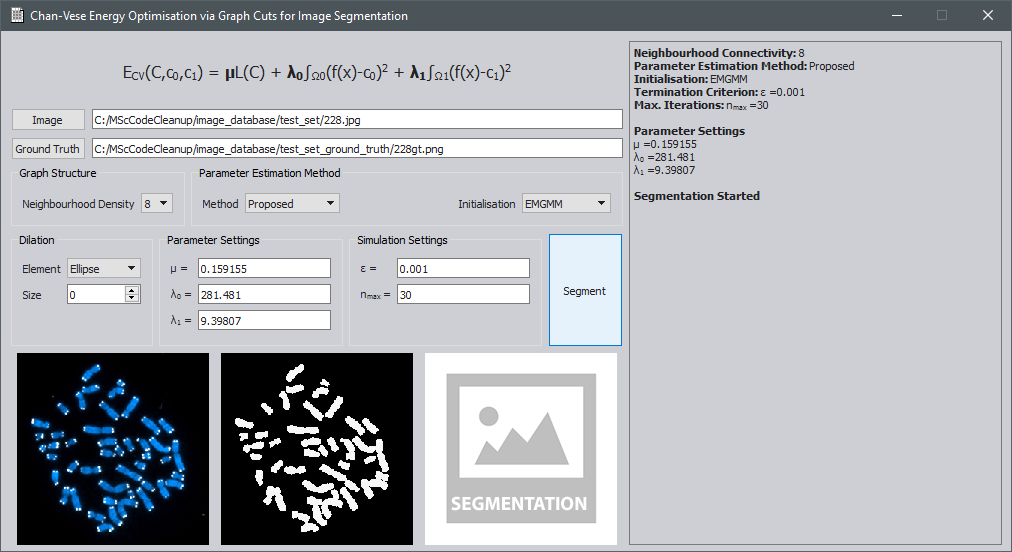
\includegraphics[width=0.90\columnwidth]{CVParamsEstimationGUI/OnSegmentationStart}
\caption{Initial segmentation summary.}
\end{figure}

\item
When the segmentation is complete, the segmentation image result will appear in its designated slot and the binary classification statistics, if a ground truth image is available, will be shown in the segmentation results box as shown in the figure below.
\begin{figure}[t]
\centering
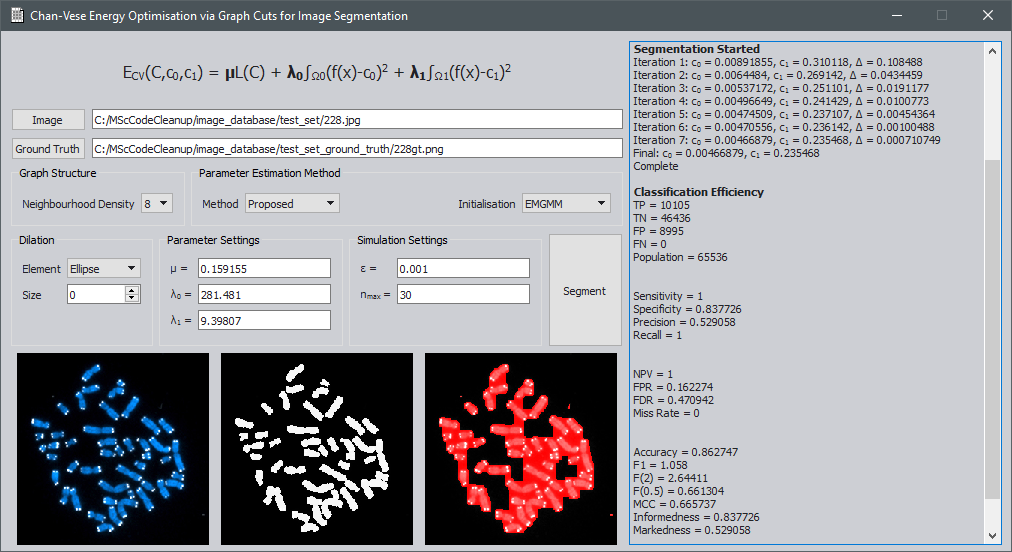
\includegraphics[width=0.90\columnwidth]{CVParamsEstimationGUI/OnSegmentationComplete}
\caption{Final segmentation results.}
\end{figure}
\end{enumerate}

\textit{Note}\\
\textit{The GUI version is buggy and impacts the segmentation process which sometimes produces inaccurate results.}

%%%%%%%%%%%%%%%%%%%%%%%%%%%%%%%%%%%%%%%%%%%%%%%%%%%%%%%%%%%%%%%%%%%%%%%%%%%%%%%%%%%%%
%%%%%%%%%%%%%%%%%%%%%%%%%%%%%%%%%%%%%%%%%%%%%%%%%%%%%%%%%%%%%%%%%%%%%%%%%%%%%%%%%%%%%
%%%%%%%%%%%%%%%%%%%%%%%%%%%%%%%%%%%%%%%%%%%%%%%%%%%%%%%%%%%%%%%%%%%%%%%%%%%%%%%%%%%%%
\clearpage
\section{Parameter Estimation for Chan-Vese Segmentation for Fluorescence Microscopy CLI}
\begin{enumerate}
\item Load in an image by giving the direct path.
\begin{figure}[h]
	\centering
	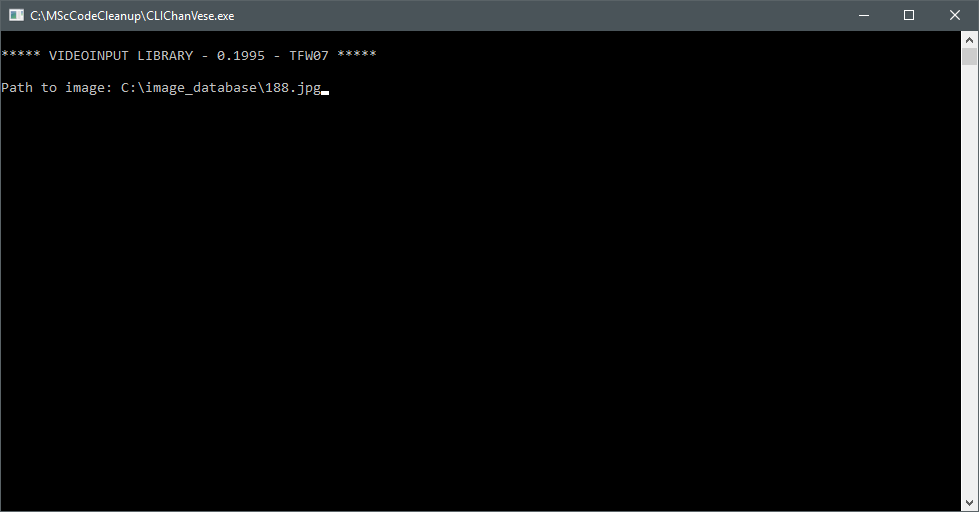
\includegraphics[width=0.90\columnwidth]{CVParamsEstimationCLI/1}
	\caption{Load image.}
\end{figure}

\item The initial mask/curve to deform is set by typing in on of the following: \textsf{default, otsu, kmeans, emgmm}.
\begin{figure}[h]
	\centering
	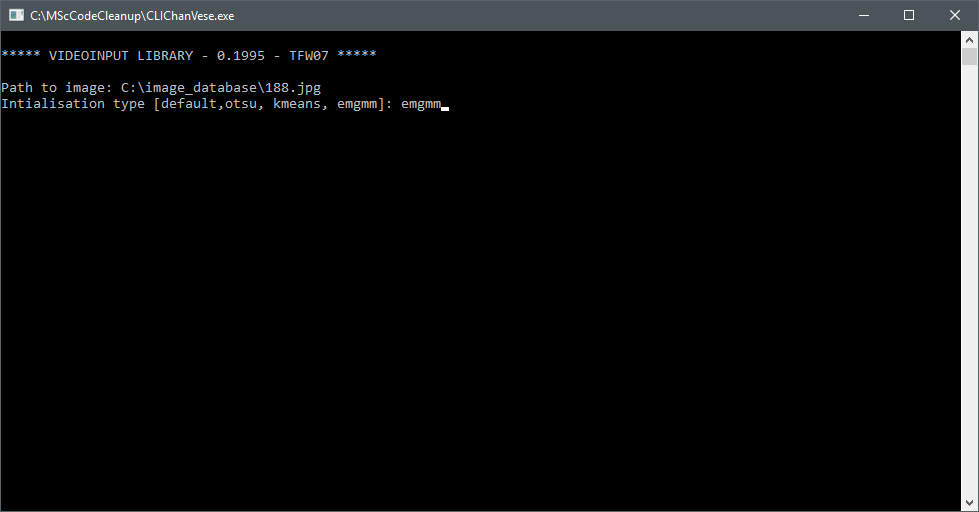
\includegraphics[width=0.90\columnwidth]{CVParamsEstimationCLI/2}
	\caption{Set initialisation method.}
\end{figure}

\item Set the dilation size. Enter a number between $0$(no dilation)-$10$.
\begin{figure}[h]
	\centering
	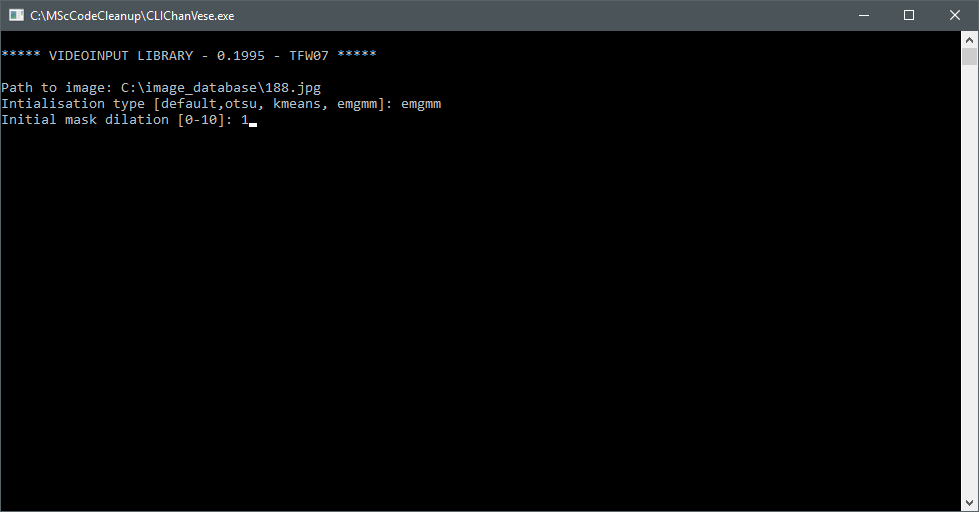
\includegraphics[width=0.90\columnwidth]{CVParamsEstimationCLI/3}
	\caption{Set mask dilation size.}
\end{figure}

\newpage
\item Set the parameter estimation method by typing in one of the following: \textsf{proposed, el-zehiry, masaka}
\begin{figure}[h]
	\centering
	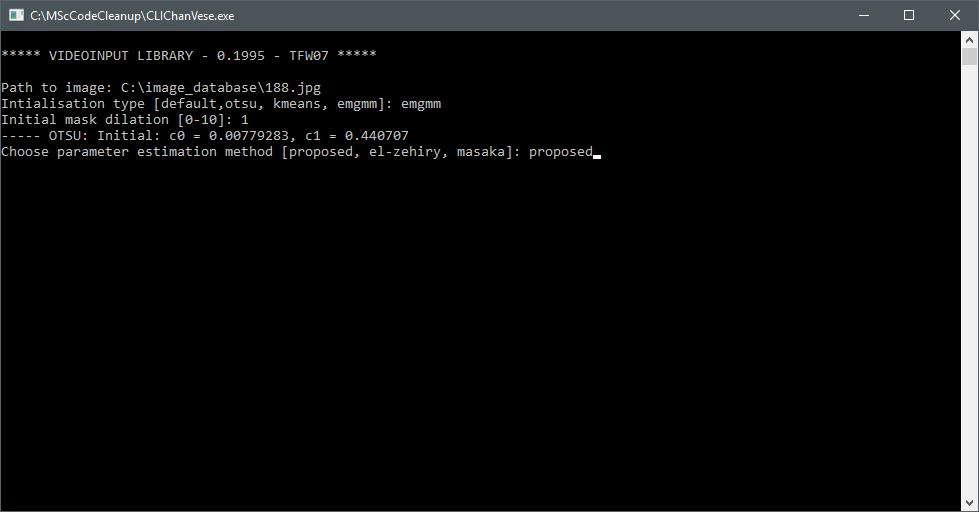
\includegraphics[width=0.90\columnwidth]{CVParamsEstimationCLI/4}
	\caption{Set parameter estimation method.}
\end{figure}

\item Set the output type. The options are \textsf{mask} or \textsf{contour}.
\begin{figure}[h]
	\centering
	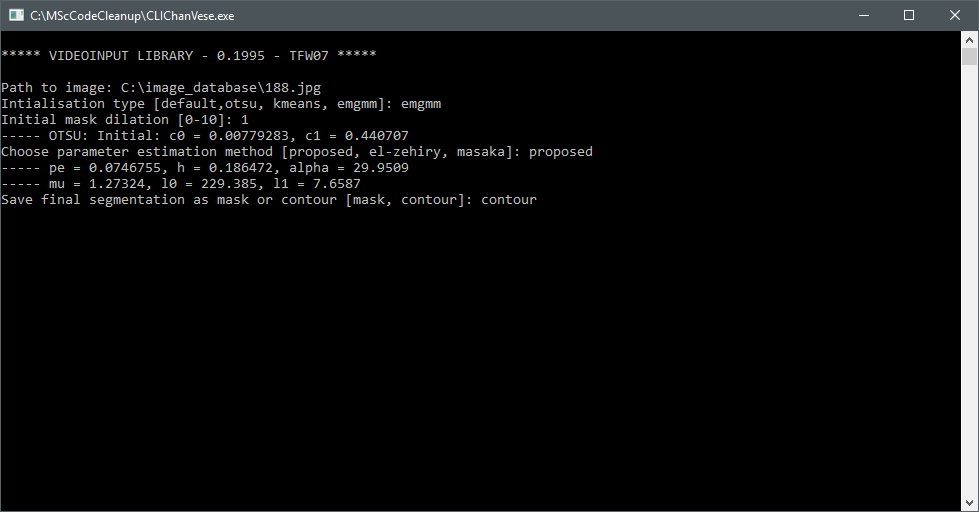
\includegraphics[width=0.90\columnwidth]{CVParamsEstimationCLI/5}
	\caption{Set final segmentation output style.}
\end{figure}

\newpage
\item If the parameters are correct then the segmentation will start successfully as shown in the figure below.
\begin{figure}[h]
	\centering
	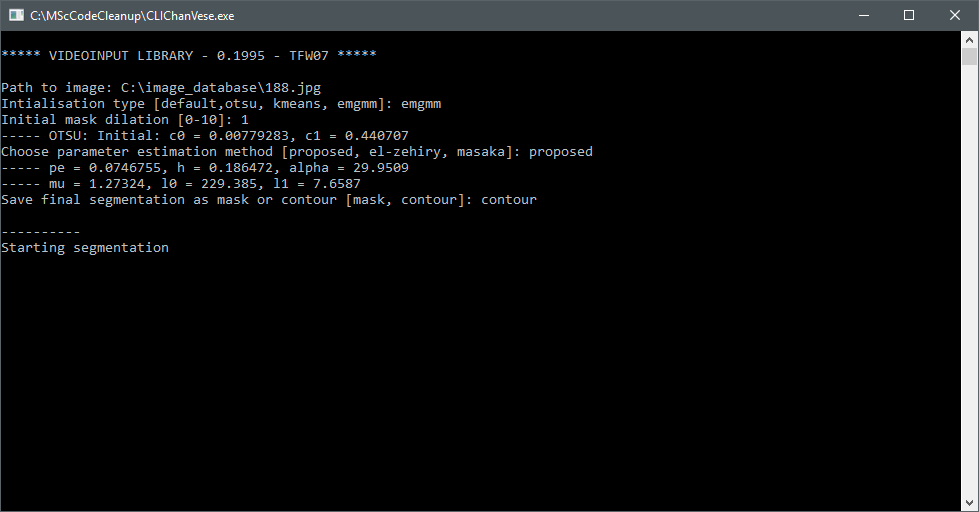
\includegraphics[width=0.90\columnwidth]{CVParamsEstimationCLI/6}
	\caption{Segmentation initialised.}
\end{figure}

\item When the segmentation is complete, the results will appear in its own window as shown in the figure below.
\begin{figure}[h]
	\centering
	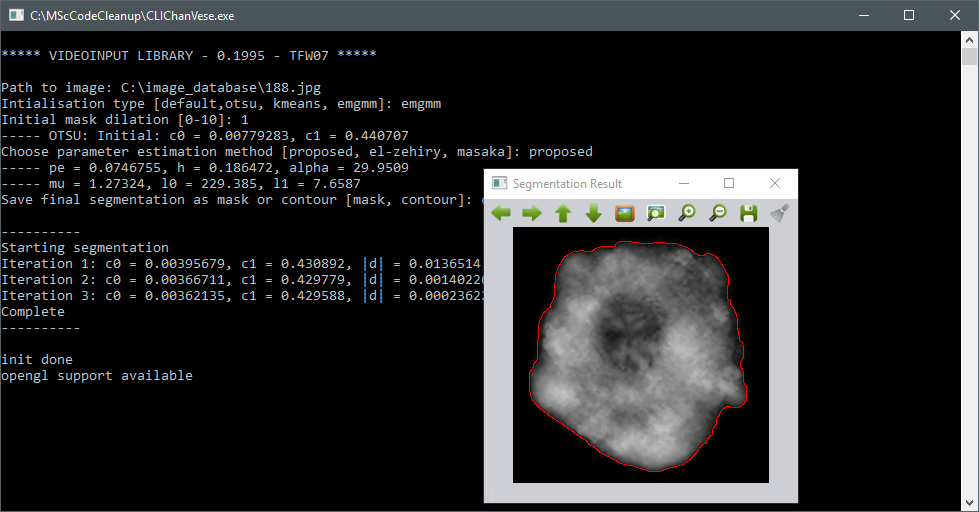
\includegraphics[width=0.90\columnwidth]{CVParamsEstimationCLI/7}
	\caption{Segmentation output.}
\end{figure}
\end{enumerate}

%%%%%%%%%%%%%%%%%%%%%%%%%%%%%%%%%%%%%%%%%%%%%%%%%%%%%%%%%%%%%%%%%%%%%%%%%%%%%%%%%%%%%
%%%%%%%%%%%%%%%%%%%%%%%%%%%%%%%%%%%%%%%%%%%%%%%%%%%%%%%%%%%%%%%%%%%%%%%%%%%%%%%%%%%%%
%%%%%%%%%%%%%%%%%%%%%%%%%%%%%%%%%%%%%%%%%%%%%%%%%%%%%%%%%%%%%%%%%%%%%%%%%%%%%%%%%%%%%
\clearpage
\section{Interactive Segmentation CLI}
\begin{enumerate}
\item Load in an image by giving the direct path as shown in the figure below.
	\begin{figure}[h]
		\centering
		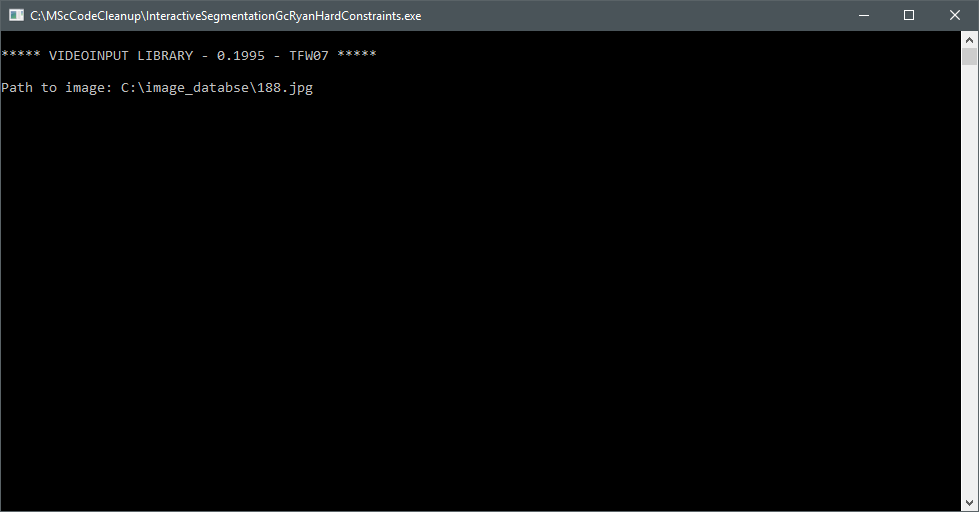
\includegraphics[width=0.9\columnwidth]{Interactive/1}
		\caption{Load in an image.}
	\end{figure}

\item Load in a seed by giving the direct path or type "x" for no seed as shown in the figure below.
\begin{figure}[h]
	\centering
	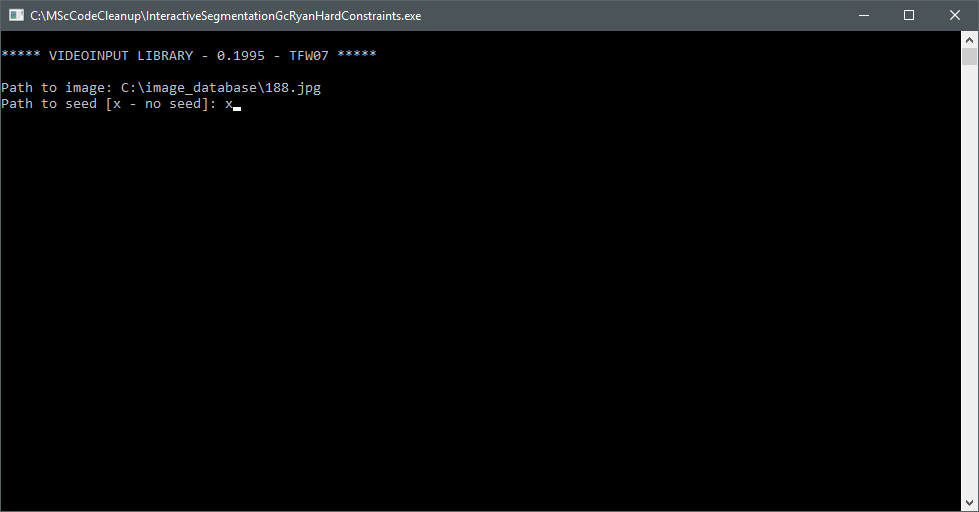
\includegraphics[width=0.90\columnwidth]{Interactive/2}
	\caption{Load in an iamge.}
\end{figure}

\item Type "y" to enable or "n" to disable real time probability distribution update as shown in the figure below.
\begin{figure}[h]
	\centering
	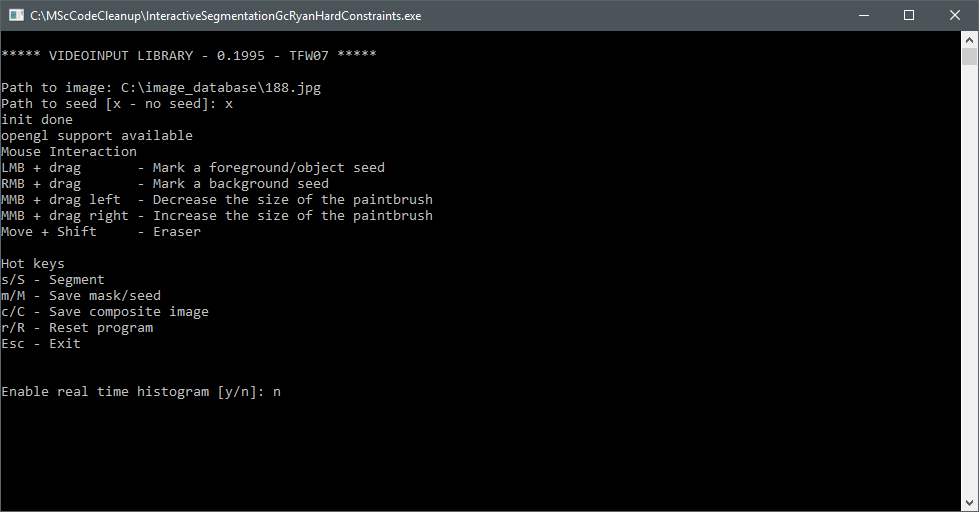
\includegraphics[width=0.90\columnwidth]{Interactive/3}
	\caption{Load in a seed.}
\end{figure}

\newpage
\item Mark object seed by left-click and dragging over the object.
\begin{figure}[h]
	\centering
	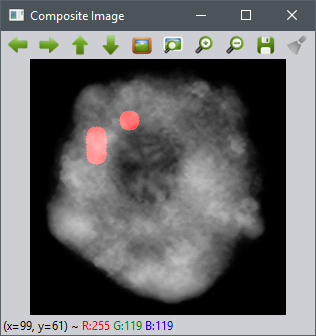
\includegraphics[width=0.50\columnwidth]{Interactive/4_1}
	\caption{Mark object.}
\end{figure}

\item Mark background seed by right-click and dragging over the object.
\begin{figure}[h]
	\centering
	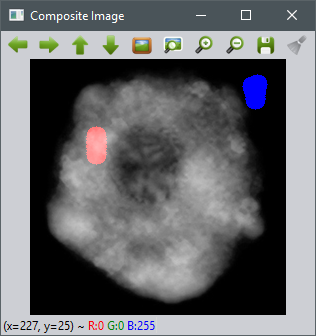
\includegraphics[width=0.50\columnwidth]{Interactive/4_2}
	\caption{Background object.}
\end{figure}

\newpage
\item \textit{Optional}. To save the seed, press "m" or "M".
\begin{figure}[h]
	\centering
	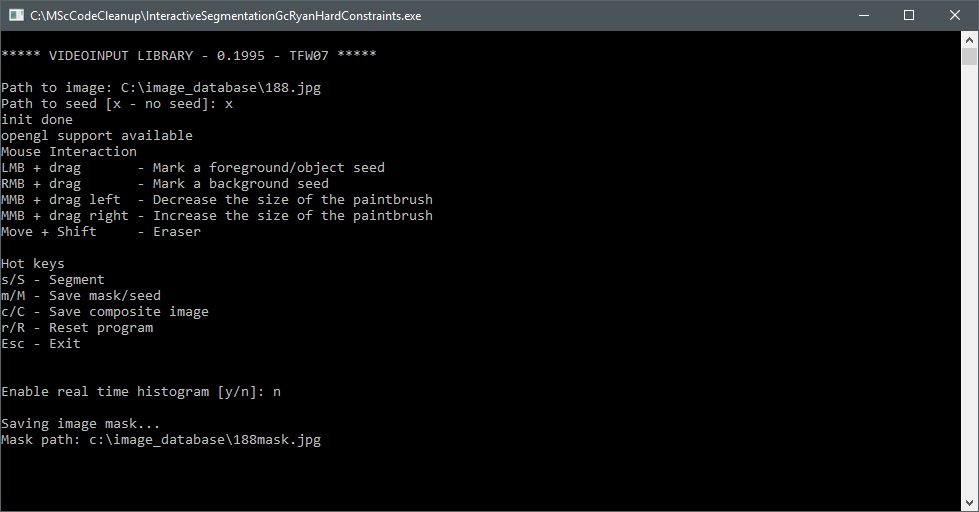
\includegraphics[width=0.90\columnwidth]{Interactive/5}
	\caption{Save seed.}
\end{figure}

\item Start segmentation by typing "s" or "S" and enter.
\begin{figure}[h]
	\centering
	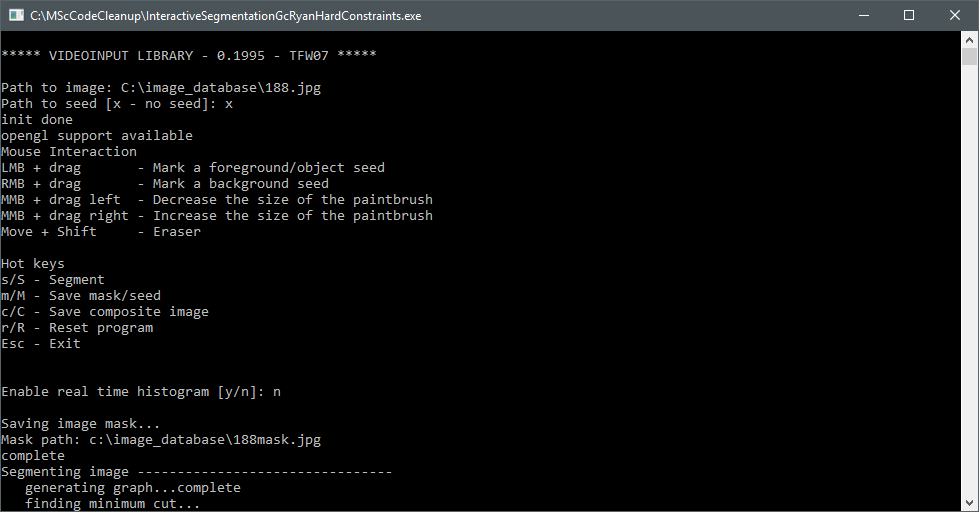
\includegraphics[width=0.90\columnwidth]{Interactive/6}
	\caption{Start segmentation.}
\end{figure}

\newpage
\item When the segmentation is complete the result will appear in the imge window as shown in the figure below. The final result can be save by pressing "c" or "C".
\begin{figure}[h]
	\centering
	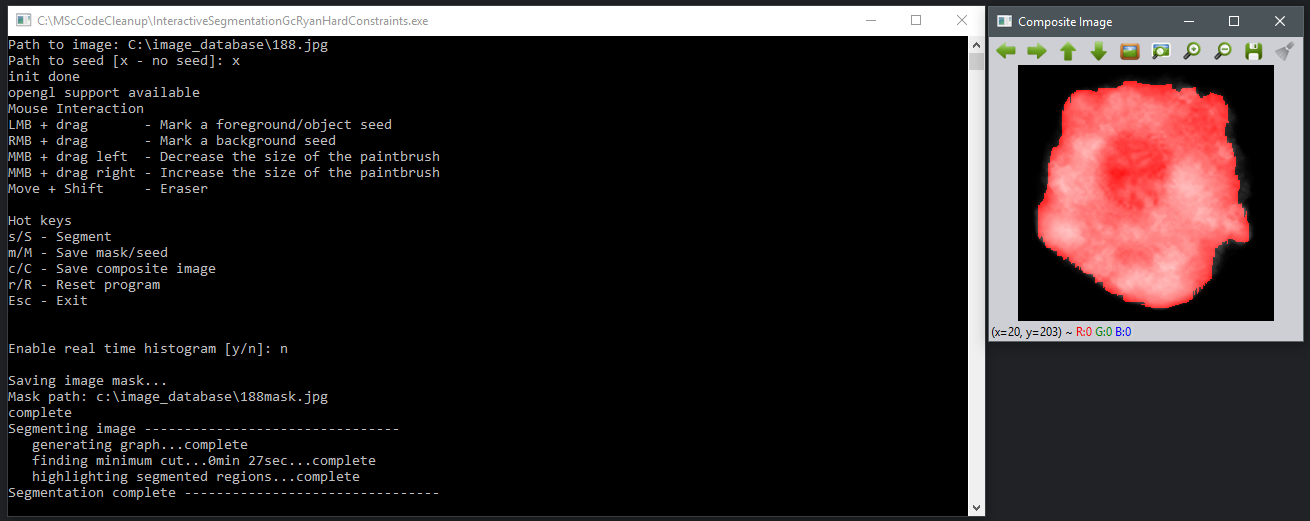
\includegraphics[width=1\columnwidth]{Interactive/7}
	\caption{Segmentation complete.}
\end{figure}
\end{enumerate}

\textit{Note}\\
\textit{Additional functionality such as increasing or decreasing brush size, erasing seeds, and resetting the program are shown in the menu.}

%%%%%%%%%%%%%%%%%%%%%%%%%%%%%%%%%%%%%%%%%%%%%%%%%%%%%%%%%%%%%%%%%%%%%%%%%%%%%%%%%%%%%
%%%%%%%%%%%%%%%%%%%%%%%%%%%%%%%%%%%%%%%%%%%%%%%%%%%%%%%%%%%%%%%%%%%%%%%%%%%%%%%%%%%%%
%%%%%%%%%%%%%%%%%%%%%%%%%%%%%%%%%%%%%%%%%%%%%%%%%%%%%%%%%%%%%%%%%%%%%%%%%%%%%%%%%%%%%
\clearpage
\section{Preprocessing Scheme}
\begin{enumerate}
	\item
	Total variation denoising is performed separately in PreprocessingScheme$\setminus$main.m. This will prompt you to search for the desired image as shown in the figure below.
	\begin{figure}[h]
		\centering
		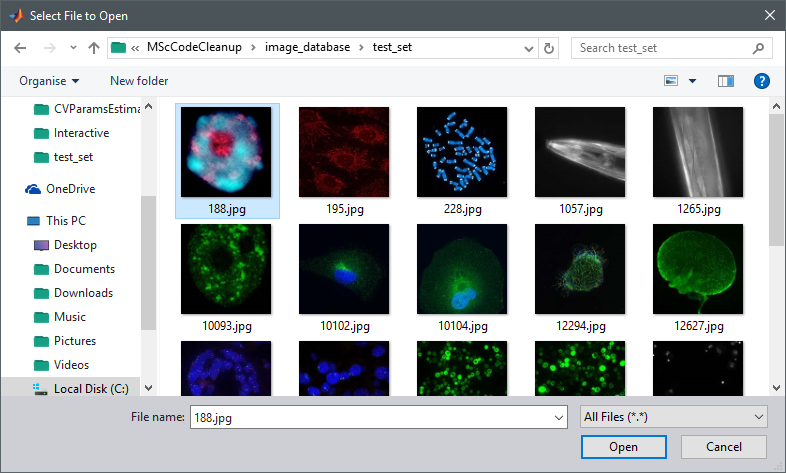
\includegraphics[width=0.9\columnwidth]{Preprocess/1}
		\caption{Load in an image.}
	\end{figure}
	
	\item The denoising effect by entering a value for gamma as shown in the figure below.
	\begin{figure}[h]
		\centering
		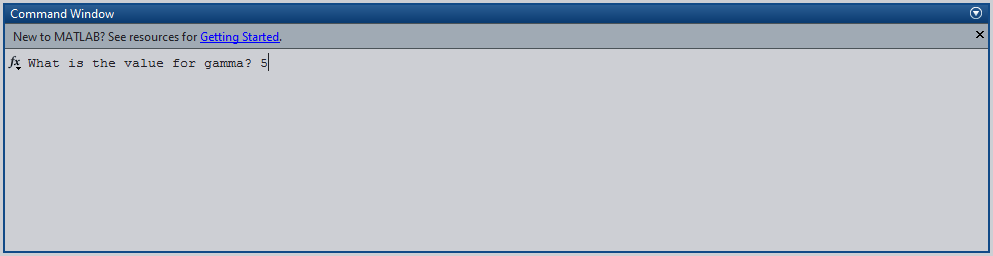
\includegraphics[width=0.90\columnwidth]{Preprocess/2}
		\caption{Set gamma.}
	\end{figure}
	
	\item Denoising is then performed on each channel in the image as shown below and combined into a single image. This image is save in the same directory as the input image and is named "tv.jpg".
	\begin{figure}[h]
		\centering
		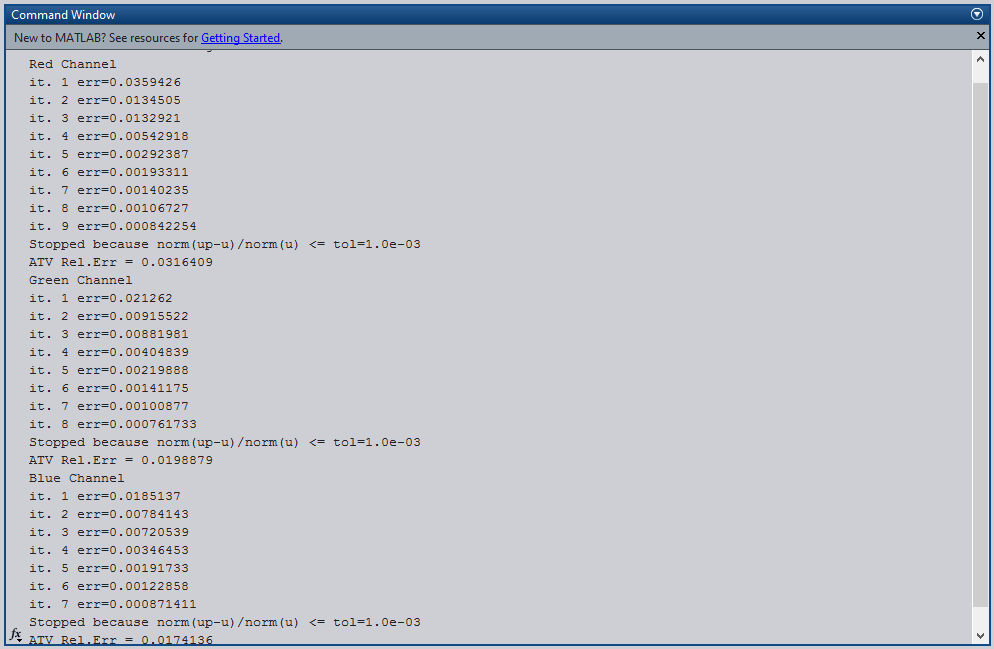
\includegraphics[width=0.90\columnwidth]{Preprocess/3}
		\caption{TV denoisong on each channel.}
	\end{figure}
	
	\newpage
%	\item ccc.
%	\begin{figure}[h]
%		\centering
%		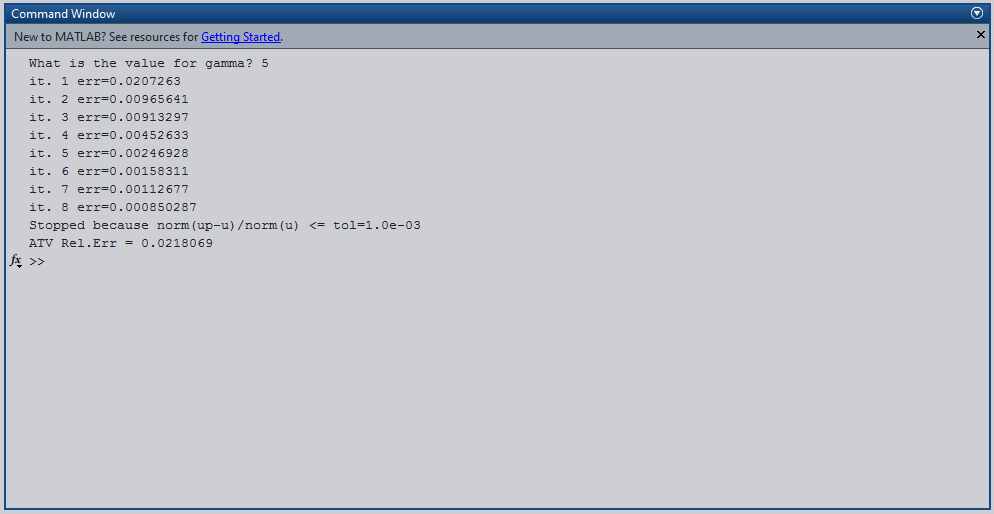
\includegraphics[width=0.50\columnwidth]{Preprocess/4}
%		\caption{Mark object.}
%	\end{figure}
%	
	\item The remainder of the preprocessing scheme is performed using\\ PreprocessingScheme$\setminus$FMPreprocessingScheme.exe. Enter the path where the total variation denoised image is as shown in the figure below.
	\begin{figure}[h]
		\centering
		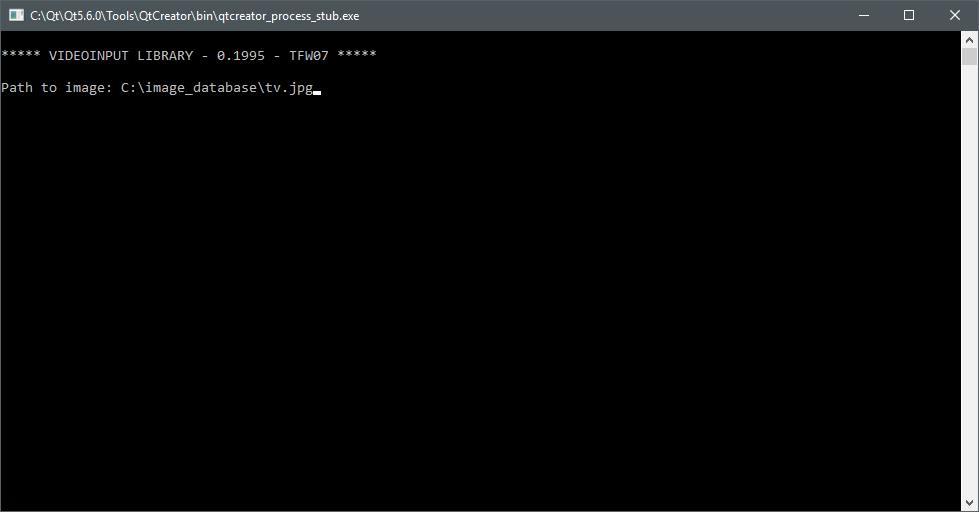
\includegraphics[width=0.90\columnwidth]{Preprocess/5}
		\caption{Background object.}
	\end{figure}
	
	\item Set the parameters for the remapping function as shown in the figure below.
	\begin{figure}[h]
		\centering
		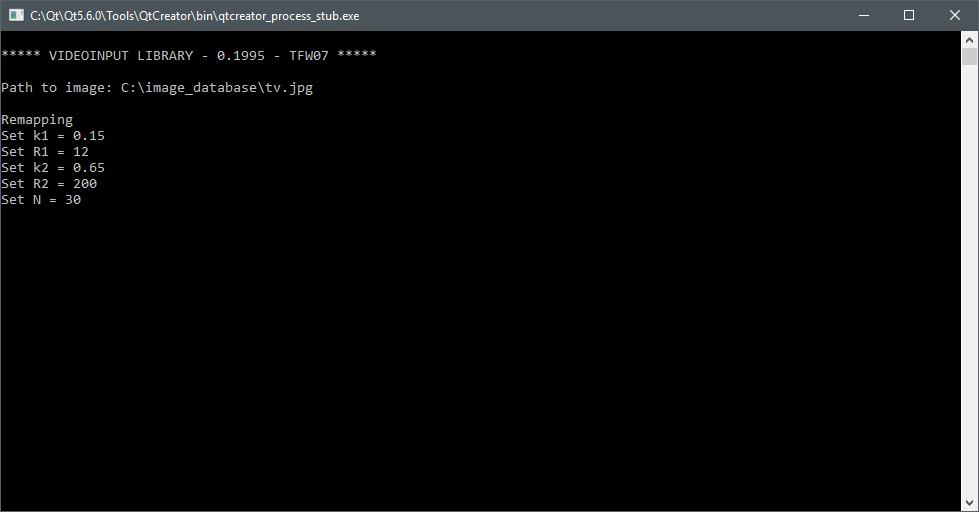
\includegraphics[width=0.90\columnwidth]{Preprocess/6}
		\caption{Remap function parameters.}
	\end{figure}
	\newpage
	\item Set the coherence enhancing diffusion parameter with optimised rotational invariance parameters as shown in the figure below.
	\begin{figure}[h]
		\centering
		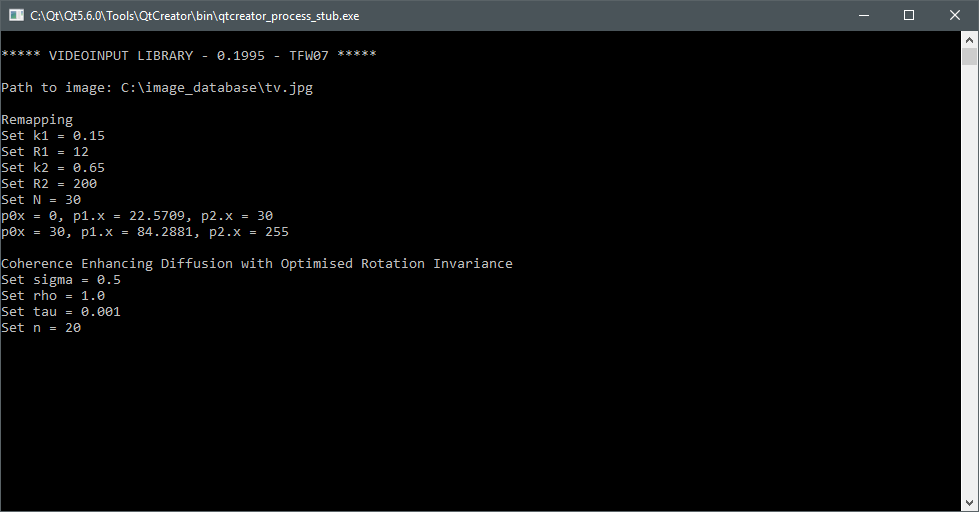
\includegraphics[width=0.90\columnwidth]{Preprocess/7}
		\caption{CEDORI parameters.}
	\end{figure}
	
	\item The final image will appear in its own window.
	\begin{figure}[h]
		\centering
		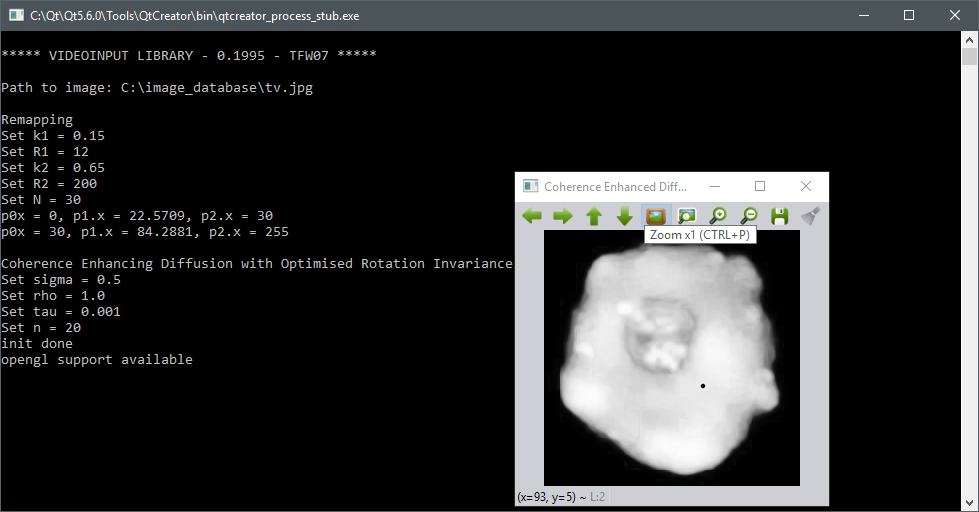
\includegraphics[width=1\columnwidth]{Preprocess/8}
		\caption{Image enhancement complete.}
	\end{figure}
\end{enumerate}


%----------------------------------------------------------------------------------------
%	BIBLIOGRAPHY
%----------------------------------------------------------------------------------------

%\renewcommand{\refname}{\spacedlowsmallcaps{References}} % For modifying the bibliography heading

%\bibliographystyle{unsrt}

%\bibliography{sample.bib} % The file containing the bibliography

%----------------------------------------------------------------------------------------

\end{document}